\chapter{Projeto Conceitual do Produto}

\section{Características gerais}

\textcolor{red}{Descrever produto de forma geral. Apresentar itens teóricos sobre o projeto a serem aprofundados ou detalhados oportunamente.}

\textcolor{red}{Apresentar e explicar a Estrutura Analítica do Projeto (EAP), tomando cuidado com a legibilidade da imagem. Se necessário, coloque a EAP dentro do comando ``\textsf{\textbackslash begin\{landscape\} \textbackslash end\{landscape\}}'' para que ela seja apresentada em uma página deitada.}

\section{Estrutura}

\textcolor{red}{Apresentar desenho em CAD, indicar dimensões por lado/aresta/cota, indicar materiais utilizados e explicar o desenho e as decisões de projeto.}

\section{Descrição de \textit{hardware}}

\textcolor{red}{A descrição de \textit{hardware} no documento deve permitir que outras pessoas repliquem o produto proposto neste documento. Para isso, deve-se explicar de forma textual os principais sub-sistemas e as escolhas de projeto, além de indicar:}

\begin{itemize}
    \item \textcolor{red}{ O diagrama de blocos \cite{blockdiagram}, que oferece uma visão geral do hardware, com as principais partes do sistema e as ligações entre elas.}
    %\item A lista de materiais \cite{bom}, que facilita a montagem do sistema, indicando tudo que deve ser adquirido. Aproveitem a lista de materiais para apresentarem o orçamento dos mesmos.
    \item \textcolor{red}{ O esquemático \cite{esquematico}, que mostra as conexões elétricas entre os componentes. Deve-se indicar os componentes por nomes e símbolos, e as conexões entre eles, incluindo a pinagem dos componentes. Se o esquemático ficar muito grande, pode-se separa-lo em vários esquemáticos. A ligação em \textit{protoboard} não é considerada um esquemático adequado.}
\end{itemize}}

\textcolor{red}{A Fig. \ref{fig:diagrama_blocos_e_esquematico} apresenta o diagrama de blocos e o esquemático de um circuito conversor de corrente alternada para corrente direta, a título de exemplo. Repare que o diagrama de blocos indica os sub-sistemas do circuito completo apresentado no esquemático. 
% Comecem com o diagrama de blocos, que é mais genérico, e depois indiquem os detalhes com a lista de materiais e os esquemáticos.
}

\begin{figure}
    \centering
    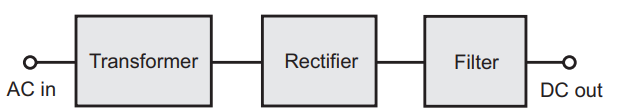
\includegraphics[width=0.5\linewidth]{figuras/Exemplo-diagrama-de-blocos.png}
    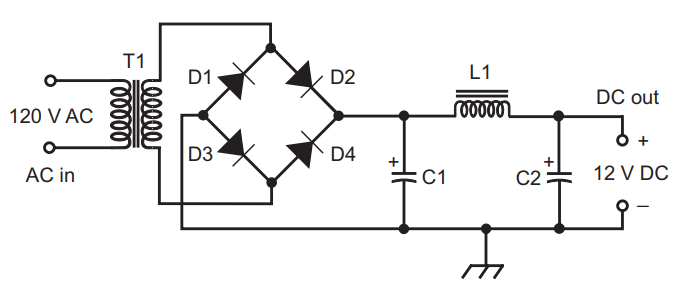
\includegraphics[width=0.5\linewidth]{figuras/Esquematico.png}
    \caption{\textcolor{red}{Diagrama de blocos e esquemático de um circuito conversor de corrente alternada para corrente direta. Extraído de \cite{block_n_schematic}.}}
    \label{fig:diagrama_blocos_e_esquematico}
\end{figure}

\section{Análise de consumo energético}

\textcolor{red}{Com relação ao consumo energético do produto desenvolvido, será necessário apresentar cálculos de consumo dos diversos componentes utilizados e explicar as decisões de projeto para atender a estas demandas.}


\begin{itemize}
    \item \textcolor{red}{ \textbf{Identificação dos Subsistemas Elétricos:} liste todos os componentes que consumirão energia, como sensores, microcontroladores, atuadores e módulos de armazenamento de dados. Para cada componente, registre a tensão de operação (V), corrente média (mA) e tempo estimado de uso (s).}
    \item \textcolor{red}{ \textbf{Cálculo da Energia Consumida por Componente:} utilize a fórmula: $E = V I t$, onde $E$ é a energia em joules, $V$ é a tensão em volts, $I$ a corrente em ampères e $t$ o tempo em segundos. Realize esse cálculo para cada componente do sistema.}
    \item \textcolor{red}{ \textbf{Estimativa do Consumo Total de Energia:} some as energias de todos os componentes para obter o consumo energético total estimado do sistema por lançamento.}
    \item \textcolor{red}{ \textbf{Escolha da Fonte de Alimentação:} com base no consumo total, converta para watt-hora: 1 Wh = 3600 J. Adicione e justifique uma margem de segurança (pesquisar o que é usual para este tipo de sistema) e selecione uma bateria ou fonte que supra a demanda.}
    \item \textcolor{red}{ \textbf{Planejamento do Circuito de Alimentação:} analise a necessidade de inclusão de reguladores de tensão, proteções contra sobrecorrente, e isolamento para atuadores. Como as oscilações de tensão serão controladas?}
    \item \textcolor{red}{ \textbf{Monitoramento via \textit{software}:} implemente, no \textit{software} embarcado, rotinas para medir a tensão da bateria e registrar dados de tempo de operação. Colete os dados para análise.}
    \item \textcolor{red}{ \textbf{Validação com Testes Reais:} realize testes de campo para comparar o consumo estimado com o real. Ajuste a capacidade da fonte se necessário e refine o software de coleta de dados. Justifique a diferença de resultados (real x teórica), de acordo com a literatura.}
\end{itemize}

\section{Descrição de \textit{software}}

\textcolor{red}{Itens fundamentais:}

\begin{itemize}
    \item \textcolor{red}{ \textbf{Diagrama BPMN para entender o \textit{software} proposto:} deve deixar claro os principais atores do sistema, suas atividades (de negócios), insumos e resultados.}
    \item \textcolor{red}{\textbf{\textit{Backlog} funcional do \textit{software}:}}
    \begin{itemize}
        \item \textcolor{red}{ Escrito no formato de histórias de usuário ou casos de uso (decisão da equipe);}
        \item \textcolor{red}{ Ao declarar o \textit{backlog} de requisitos funcionais, usar a  classificação de MoSCoW (\textit{Must have}, \textit{Should have} e \textit{Could have}),  para um melhor entendimento do próprio \textit{backlog}.}
    \end{itemize}
    \item \textcolor{red}{\textbf{ \textit{Backlog} não-funcional do \textit{software}:}}
    \begin{itemize}
        \item \textcolor{red}{ Descrever os requisitos não-funcionais de forma objetiva;}
        \item \textcolor{red}{ Mais facilmente, mais rapidamente, são descrições subjetivas não-válidas. Um exemplo de requisito não-funcional de desempenho: ``a página deve carregar em até 5s quando em conexão 4G''. }
    \end{itemize}
    \item \textcolor{red}{ \textbf{Diagrama de casos de uso,} contendo os atores do sistema, os requisitos com os quais eles interagem e os tipos de relacionamentos entre requisitos realizados por um mesmo ator (ex.: \textit{include}, \textit{extend}). Obs.: este é um diagrama sobre requisitos funcionais.}
    \item \textcolor{red}{ \textbf{Descrição da arquitetura da solução de \textit{software} proposta:}}
    \begin{itemize}
        \item \textcolor{red}{ Propósito do \textit{software} (qual o seu papel no sistema);}
        \item \textcolor{red}{ Estilo arquitetural contendo:}
        \begin{itemize}
            \item \textcolor{red}{ Padrão adotado: MVC, MVP, Microsserviços, Monolítico, etc (Justificar);}
            \item \textcolor{red}{ Linguagens de programação: Java, Python, C\#, JavaScript, etc.}
            \item \textcolor{red}{ \textit{Frameworks} e bibliotecas: Spring Boot, .NET Core, React, Angular, Django, etc.}
            \item \textcolor{red}{ Banco de dados: Relacional (PostgreSQL, MySQL, etc) X NãoSQL (MongoDB,etc). }
        \end{itemize}
        \item \textcolor{red}{ Diagrama de alto nível: representação esquemática dos componentes da arquitetura, suas responsabilidades e comunicações, esclarecendo a composição do \textit{front-end} e do \textit{back-end}.}
    \end{itemize}
    \item \textcolor{red}{ \textbf{Persistência de dados:} diagrama de entidade relacionamento do banco de dados usado na solução proposta.}
    \item \textcolor{red}{ \textbf{Análise de dados:} as variáveis definidas nos requisitos do projeto em abordagem numérica e gráfica.}
    \item \textcolor{red}{ \textbf{Diagrama de estados} esclarecendo os estados assumidos pelo \textit{software} e os eventos que causam as mudanças de estado do \textit{software}.}
    \item \textcolor{red}{ \textbf{Protótipo funcional do \textit{software}, navegável.}}
    \item \textcolor{red}{\textbf{ Roteiro de testes funcionais:} }
    \begin{itemize}
        \item \textcolor{red}{Código do caso de teste;}
        \item \textcolor{red}{Nome do caso de teste;}
        \item \textcolor{red}{Tipo do caso de teste (unitário, integrado ou sistema);}
        \item \textcolor{red}{ Objetivo do caso de teste;}
        \item \textcolor{red}{ Pré-condições do sistema para o teste ser realizado;}
        \item \textcolor{red}{ Descrição dos procedimentos a serem executados para o teste;}
        \item \textcolor{red}{ Resultado esperado para o teste ser aprovado (pós-condição após realizado o teste);}
        \item \textcolor{red}{ Especificação do reparo a ser executado (caso o teste não seja aprovado);}
        \item \textcolor{red}{ Resultado após reparo (o caso do teste ser necessário de ser repetido após reparo).}
    \end{itemize}
\end{itemize}


% \textcolor{red}{Com relação ao \textit{software}, será necessário apresentar os seguintes itens: % pacotes de componentes de \textit{software}, suas funções e características, e explicar as decisões de projeto:
% \begin{enumerate}
%     \item Um diagrama do processo de negócio do problema que a máquina se propõe a resolver (BPNM) – não é UML, mas é fundamental para entender como o sistema se comporta como um todo, incluindo o usuário;
%     \item Lista de casos de uso (backlog do sistema). Backlog funcional;
%     \item Lista de requisitos não-funcionais a serem satisfeitos pelo sistema;
%     \item Diagrama de casos de uso: mostrando os requisitos funcionais, seus atores e como eles interagem entre si;
%     \item Diagrama de Classes: apresentando quais dados são manipulados pelo sistema (internamente e externamente – ex.: resultados de experimentos);
%     \item Diagrama de arquitetura, identificando todos os componentes da máquina e suas iterações com o software;
%     \item Diagrama de estados da máquina (sistema);
%     \item Descrição dos testes dos componentes da máquina e dos testes funcionais que deveriam ser feitos para avaliar o funcionamento da máquina e identificar defeitos. São importantes os testes unitários (componentes) e de integração (conjunto de componentes) e o roteiro de testes.
% \end{enumerate}
% }
%\textcolor{red}{Com relação ao \textit{software}, será necessário apresentar pacotes de componentes de \textit{software}, suas funções e características, e explicar as decisões de projeto.}

